% Options for packages loaded elsewhere
\PassOptionsToPackage{unicode}{hyperref}
\PassOptionsToPackage{hyphens}{url}
%
\documentclass[
]{article}
\usepackage{amsmath,amssymb}
\usepackage{lmodern}
\usepackage{ifxetex,ifluatex}
\ifnum 0\ifxetex 1\fi\ifluatex 1\fi=0 % if pdftex
  \usepackage[T1]{fontenc}
  \usepackage[utf8]{inputenc}
  \usepackage{textcomp} % provide euro and other symbols
\else % if luatex or xetex
  \usepackage{unicode-math}
  \defaultfontfeatures{Scale=MatchLowercase}
  \defaultfontfeatures[\rmfamily]{Ligatures=TeX,Scale=1}
\fi
% Use upquote if available, for straight quotes in verbatim environments
\IfFileExists{upquote.sty}{\usepackage{upquote}}{}
\IfFileExists{microtype.sty}{% use microtype if available
  \usepackage[]{microtype}
  \UseMicrotypeSet[protrusion]{basicmath} % disable protrusion for tt fonts
}{}
\makeatletter
\@ifundefined{KOMAClassName}{% if non-KOMA class
  \IfFileExists{parskip.sty}{%
    \usepackage{parskip}
  }{% else
    \setlength{\parindent}{0pt}
    \setlength{\parskip}{6pt plus 2pt minus 1pt}}
}{% if KOMA class
  \KOMAoptions{parskip=half}}
\makeatother
\usepackage{xcolor}
\IfFileExists{xurl.sty}{\usepackage{xurl}}{} % add URL line breaks if available
\IfFileExists{bookmark.sty}{\usepackage{bookmark}}{\usepackage{hyperref}}
\hypersetup{
  pdftitle={STAT 231: Problem Set 2B},
  pdfauthor={Lorraine Oloo},
  hidelinks,
  pdfcreator={LaTeX via pandoc}}
\urlstyle{same} % disable monospaced font for URLs
\usepackage[margin=1in]{geometry}
\usepackage{color}
\usepackage{fancyvrb}
\newcommand{\VerbBar}{|}
\newcommand{\VERB}{\Verb[commandchars=\\\{\}]}
\DefineVerbatimEnvironment{Highlighting}{Verbatim}{commandchars=\\\{\}}
% Add ',fontsize=\small' for more characters per line
\usepackage{framed}
\definecolor{shadecolor}{RGB}{248,248,248}
\newenvironment{Shaded}{\begin{snugshade}}{\end{snugshade}}
\newcommand{\AlertTok}[1]{\textcolor[rgb]{0.94,0.16,0.16}{#1}}
\newcommand{\AnnotationTok}[1]{\textcolor[rgb]{0.56,0.35,0.01}{\textbf{\textit{#1}}}}
\newcommand{\AttributeTok}[1]{\textcolor[rgb]{0.77,0.63,0.00}{#1}}
\newcommand{\BaseNTok}[1]{\textcolor[rgb]{0.00,0.00,0.81}{#1}}
\newcommand{\BuiltInTok}[1]{#1}
\newcommand{\CharTok}[1]{\textcolor[rgb]{0.31,0.60,0.02}{#1}}
\newcommand{\CommentTok}[1]{\textcolor[rgb]{0.56,0.35,0.01}{\textit{#1}}}
\newcommand{\CommentVarTok}[1]{\textcolor[rgb]{0.56,0.35,0.01}{\textbf{\textit{#1}}}}
\newcommand{\ConstantTok}[1]{\textcolor[rgb]{0.00,0.00,0.00}{#1}}
\newcommand{\ControlFlowTok}[1]{\textcolor[rgb]{0.13,0.29,0.53}{\textbf{#1}}}
\newcommand{\DataTypeTok}[1]{\textcolor[rgb]{0.13,0.29,0.53}{#1}}
\newcommand{\DecValTok}[1]{\textcolor[rgb]{0.00,0.00,0.81}{#1}}
\newcommand{\DocumentationTok}[1]{\textcolor[rgb]{0.56,0.35,0.01}{\textbf{\textit{#1}}}}
\newcommand{\ErrorTok}[1]{\textcolor[rgb]{0.64,0.00,0.00}{\textbf{#1}}}
\newcommand{\ExtensionTok}[1]{#1}
\newcommand{\FloatTok}[1]{\textcolor[rgb]{0.00,0.00,0.81}{#1}}
\newcommand{\FunctionTok}[1]{\textcolor[rgb]{0.00,0.00,0.00}{#1}}
\newcommand{\ImportTok}[1]{#1}
\newcommand{\InformationTok}[1]{\textcolor[rgb]{0.56,0.35,0.01}{\textbf{\textit{#1}}}}
\newcommand{\KeywordTok}[1]{\textcolor[rgb]{0.13,0.29,0.53}{\textbf{#1}}}
\newcommand{\NormalTok}[1]{#1}
\newcommand{\OperatorTok}[1]{\textcolor[rgb]{0.81,0.36,0.00}{\textbf{#1}}}
\newcommand{\OtherTok}[1]{\textcolor[rgb]{0.56,0.35,0.01}{#1}}
\newcommand{\PreprocessorTok}[1]{\textcolor[rgb]{0.56,0.35,0.01}{\textit{#1}}}
\newcommand{\RegionMarkerTok}[1]{#1}
\newcommand{\SpecialCharTok}[1]{\textcolor[rgb]{0.00,0.00,0.00}{#1}}
\newcommand{\SpecialStringTok}[1]{\textcolor[rgb]{0.31,0.60,0.02}{#1}}
\newcommand{\StringTok}[1]{\textcolor[rgb]{0.31,0.60,0.02}{#1}}
\newcommand{\VariableTok}[1]{\textcolor[rgb]{0.00,0.00,0.00}{#1}}
\newcommand{\VerbatimStringTok}[1]{\textcolor[rgb]{0.31,0.60,0.02}{#1}}
\newcommand{\WarningTok}[1]{\textcolor[rgb]{0.56,0.35,0.01}{\textbf{\textit{#1}}}}
\usepackage{graphicx}
\makeatletter
\def\maxwidth{\ifdim\Gin@nat@width>\linewidth\linewidth\else\Gin@nat@width\fi}
\def\maxheight{\ifdim\Gin@nat@height>\textheight\textheight\else\Gin@nat@height\fi}
\makeatother
% Scale images if necessary, so that they will not overflow the page
% margins by default, and it is still possible to overwrite the defaults
% using explicit options in \includegraphics[width, height, ...]{}
\setkeys{Gin}{width=\maxwidth,height=\maxheight,keepaspectratio}
% Set default figure placement to htbp
\makeatletter
\def\fps@figure{htbp}
\makeatother
\setlength{\emergencystretch}{3em} % prevent overfull lines
\providecommand{\tightlist}{%
  \setlength{\itemsep}{0pt}\setlength{\parskip}{0pt}}
\setcounter{secnumdepth}{-\maxdimen} % remove section numbering
\ifluatex
  \usepackage{selnolig}  % disable illegal ligatures
\fi

\title{STAT 231: Problem Set 2B}
\author{Lorraine Oloo}
\date{due by 5 PM on Friday, March 5}

\begin{document}
\maketitle

Series B homework assignments are designed to help you further ingest
and practice the material covered in class over the past week(s). You
are encouraged to work with other students, but all code must be written
by you and you must indicate below who you discussed the assignment with
(if anyone).

Steps to proceed:

\begin{_}
\item In RStudio, go to File > Open Project, navigate to the folder with the course-content repo, select the course-content project (course-content.Rproj), and click "Open" 
\item Pull the course-content repo (e.g. using the blue-ish down arrow in the Git tab in upper right window)
\item Copy ps2B.Rmd from the course repo to your repo (see page 6 of the GitHub Classroom Guide for Stat231 if needed)
\item Close the course-content repo project in RStudio
\item Open YOUR repo project in RStudio
\item In the ps2B.Rmd file in YOUR repo, replace "YOUR NAME HERE" with your name
\item Add in your responses, committing and pushing to YOUR repo in appropriate places along the way
\item Run "Knit PDF" 
\item Upload the pdf to Gradescope.  Don't forget to select which of your pages are associated with each problem.  \textit{You will not get credit for work on unassigned pages (e.g., if you only selected the first page but your solution spans two pages, you would lose points for any part on the second page that the grader can't see).} 
\end{_}

\newpage

\hypertarget{if-you-discussed-this-assignment-with-any-of-your-peers-please-list-who-here}{%
\section{If you discussed this assignment with any of your peers, please
list who
here:}\label{if-you-discussed-this-assignment-with-any-of-your-peers-please-list-who-here}}

\begin{quote}
ANSWER:
\end{quote}

\newpage

\hypertarget{mdsr-exercise-4.14-modified}{%
\section{MDSR Exercise 4.14
(modified)}\label{mdsr-exercise-4.14-modified}}

Use the \texttt{Pitching} data frame from the \texttt{Lahman} package to
identify every pitcher in baseball history who has accumulated at least
300 wins (\texttt{W}) and at least 3,000 strikeouts (\texttt{SO}).

\begin{enumerate}
\def\labelenumi{\alph{enumi}.}
\tightlist
\item
  How many pitchers meet this criteria?
\end{enumerate}

\begin{quote}
ANSWER: 10 pitchers meet this criteria
\end{quote}

\begin{Shaded}
\begin{Highlighting}[]
\FunctionTok{library}\NormalTok{(Lahman)}
\FunctionTok{data}\NormalTok{(}\StringTok{"Pitching"}\NormalTok{)}
\end{Highlighting}
\end{Shaded}

\begin{Shaded}
\begin{Highlighting}[]
\NormalTok{Pitching1 }\OtherTok{\textless{}{-}} \FunctionTok{select}\NormalTok{(Pitching, playerID, W, SO)}

\NormalTok{Pitching2}\OtherTok{\textless{}{-}} \FunctionTok{aggregate}\NormalTok{(}\FunctionTok{cbind}\NormalTok{(W, SO) }\SpecialCharTok{\textasciitilde{}}\NormalTok{ playerID, }\AttributeTok{data =}\NormalTok{ Pitching1, sum)}

\NormalTok{Pitching3}\OtherTok{\textless{}{-}} \FunctionTok{filter}\NormalTok{(Pitching2, W }\SpecialCharTok{\textgreater{}} \DecValTok{300} \SpecialCharTok{\&}\NormalTok{ SO }\SpecialCharTok{\textgreater{}} \DecValTok{3000}\NormalTok{)}
\NormalTok{Pitching3}
\end{Highlighting}
\end{Shaded}

\begin{verbatim}
##     playerID   W   SO
## 1  carltst01 329 4136
## 2  clemero02 354 4672
## 3  johnsra05 303 4875
## 4  johnswa01 417 3509
## 5  maddugr01 355 3371
## 6  niekrph01 318 3342
## 7  perryga01 314 3534
## 8   ryanno01 324 5714
## 9  seaveto01 311 3640
## 10 suttodo01 324 3574
\end{verbatim}

\begin{enumerate}
\def\labelenumi{\alph{enumi}.}
\setcounter{enumi}{1}
\tightlist
\item
  Which of these pitchers had the most accumulated strikeouts? How many
  strikeouts had he accumulated? What is the most strikeouts he had in
  one season?
\end{enumerate}

\begin{quote}
ANSWER: ryanno01 had the most accumulated strikeouts of 5714. The most
strikeouts he had in one season is 383.
\end{quote}

\begin{Shaded}
\begin{Highlighting}[]
\CommentTok{\#Maximum strikeout}
\NormalTok{Pitching4}\OtherTok{\textless{}{-}} \FunctionTok{filter}\NormalTok{(Pitching3, SO}\SpecialCharTok{==} \FunctionTok{max}\NormalTok{(Pitching3}\SpecialCharTok{$}\NormalTok{SO))}
\NormalTok{Pitching4}
\end{Highlighting}
\end{Shaded}

\begin{verbatim}
##   playerID   W   SO
## 1 ryanno01 324 5714
\end{verbatim}

\begin{Shaded}
\begin{Highlighting}[]
\CommentTok{\#player ryanno01 games only}
\NormalTok{Pitching5}\OtherTok{\textless{}{-}} \FunctionTok{filter}\NormalTok{(Pitching, playerID }\SpecialCharTok{==} \StringTok{"ryanno01"}\NormalTok{)}
\FunctionTok{max}\NormalTok{(Pitching5}\SpecialCharTok{$}\NormalTok{SO)}
\end{Highlighting}
\end{Shaded}

\begin{verbatim}
## [1] 383
\end{verbatim}

\newpage

\hypertarget{mdsr-exercise-4.17-modified}{%
\section{MDSR Exercise 4.17
(modified)}\label{mdsr-exercise-4.17-modified}}

\begin{enumerate}
\def\labelenumi{\alph{enumi}.}
\tightlist
\item
  The Violations data set in the \texttt{mdsr} package contains
  information regarding the outcome of health inspections in New York
  City. Use these data to calculate the median violation score by
  zipcode and dba for zipcodes in Manhattan. What pattern (if any) do
  you see between the number of inspections and the median score?
  Generate a visualization to support your response.
\end{enumerate}

\begin{quote}
ANSWER: There is a moderate positive assosiation between the number of
inspections and the median score.
\end{quote}

\begin{Shaded}
\begin{Highlighting}[]
\FunctionTok{data}\NormalTok{(}\StringTok{"Violations"}\NormalTok{)}
\NormalTok{Violations1}\OtherTok{\textless{}{-}}\NormalTok{ Violations }\SpecialCharTok{\%\textgreater{}\%} \FunctionTok{drop\_na}\NormalTok{()}
\end{Highlighting}
\end{Shaded}

\begin{Shaded}
\begin{Highlighting}[]
\NormalTok{Violation2 }\OtherTok{\textless{}{-}}\NormalTok{Violations1 }\SpecialCharTok{\%\textgreater{}\%}
  \FunctionTok{filter}\NormalTok{(boro }\SpecialCharTok{==} \StringTok{"MANHATTAN"}\NormalTok{) }\SpecialCharTok{\%\textgreater{}\%}
  \FunctionTok{select}\NormalTok{(zipcode,dba,score,)}\SpecialCharTok{\%\textgreater{}\%}
  \FunctionTok{group\_by}\NormalTok{(zipcode,dba) }\SpecialCharTok{\%\textgreater{}\%}
  \FunctionTok{summarise}\NormalTok{(}\AttributeTok{num\_inspections=}\FunctionTok{n}\NormalTok{(), }\AttributeTok{med\_score=}\FunctionTok{median}\NormalTok{(score))}
\end{Highlighting}
\end{Shaded}

\begin{verbatim}
## `summarise()` has grouped output by 'zipcode'. You can override using the `.groups` argument.
\end{verbatim}

\begin{Shaded}
\begin{Highlighting}[]
\NormalTok{g }\OtherTok{\textless{}{-}} \FunctionTok{ggplot}\NormalTok{(}\AttributeTok{data =}\NormalTok{ Violation2, }\FunctionTok{aes}\NormalTok{(}\AttributeTok{y =}\NormalTok{ med\_score, }\AttributeTok{x =}\NormalTok{ num\_inspections)) }\SpecialCharTok{+} \FunctionTok{ggtitle}\NormalTok{(}\StringTok{"Number of inspections vs the median score"}\NormalTok{) }\SpecialCharTok{+} \FunctionTok{ylab}\NormalTok{(}\StringTok{"median score"}\NormalTok{) }\SpecialCharTok{+} \FunctionTok{xlab}\NormalTok{(}\StringTok{"no. of inspections"}\NormalTok{)}
\NormalTok{g }\SpecialCharTok{+} \FunctionTok{geom\_point}\NormalTok{(}\AttributeTok{size =} \DecValTok{1}\NormalTok{)}
\end{Highlighting}
\end{Shaded}

\includegraphics{ps2B_files/figure-latex/unnamed-chunk-5-1.pdf}

\begin{enumerate}
\def\labelenumi{\alph{enumi}.}
\setcounter{enumi}{1}
\tightlist
\item
  In your visualization in part (a), there should be at least a few
  points that stand out as outliers. For \emph{one of the outliers}, add
  text to the outlier identifying what business it is and an arrow
  pointing from the text to the observation. First, you may want to
  \texttt{filter} to identify the name of the business (so you know what
  text to add to the plot).
\end{enumerate}

(Can't remember how to create a curved arrow in \texttt{ggplot}? The
answers to
\href{https://stackoverflow.com/questions/38008863/how-to-draw-a-nice-arrow-in-ggplot2/61383034}{this
question} on Stack Exchange may help. Can't remember how to add text to
the plot in \texttt{ggplot}? Check out the text examples with
\texttt{annotate}
\href{https://ggplot2.tidyverse.org/reference/annotate.html}{here}, or
answers to
\href{https://stackoverflow.com/questions/14351608/color-one-point-and-add-an-annotation-in-ggplot2/14351810}{this
question} that use \texttt{geom\_text}.)

\begin{quote}
STARBUCKS with 110 total inspections and a median of 9.
\end{quote}

\begin{Shaded}
\begin{Highlighting}[]
\CommentTok{\#filter(Violation2, num\_inspections\textgreater{}105)}

\NormalTok{context }\OtherTok{\textless{}{-}} \FunctionTok{tribble}\NormalTok{(}
  \SpecialCharTok{\textasciitilde{}}\NormalTok{num\_inspections, }\SpecialCharTok{\textasciitilde{}}\NormalTok{med\_score, }\SpecialCharTok{\textasciitilde{}}\NormalTok{label,}
  \DecValTok{90}\NormalTok{, }\DecValTok{30}\NormalTok{, }\StringTok{"Starbucks"}\NormalTok{)}

\NormalTok{g }\SpecialCharTok{+} \FunctionTok{geom\_point}\NormalTok{(}\AttributeTok{size =} \DecValTok{1}\NormalTok{) }\SpecialCharTok{+}
  \FunctionTok{geom\_text}\NormalTok{(}
    \AttributeTok{data =}\NormalTok{ context, }
    \FunctionTok{aes}\NormalTok{(}\AttributeTok{y =}\NormalTok{ med\_score, }\AttributeTok{label =}\NormalTok{ label, }\AttributeTok{color =}\NormalTok{ label)}
\NormalTok{  ) }\SpecialCharTok{+} 
  \FunctionTok{geom\_curve}\NormalTok{(}
    \AttributeTok{x =} \DecValTok{90}\NormalTok{, }\AttributeTok{xend =} \DecValTok{110}\NormalTok{, }\AttributeTok{y =} \DecValTok{30}\NormalTok{, }\AttributeTok{yend =} \FloatTok{10.5}\NormalTok{, }
    \AttributeTok{arrow =} \FunctionTok{arrow}\NormalTok{(}\AttributeTok{length =} \FunctionTok{unit}\NormalTok{(}\FloatTok{0.2}\NormalTok{, }\StringTok{"cm"}\NormalTok{)), }\AttributeTok{curvature =} \SpecialCharTok{{-}}\FloatTok{0.5}
\NormalTok{  ) }\SpecialCharTok{+} 
  \FunctionTok{scale\_color\_manual}\NormalTok{(}
    \AttributeTok{guide =} \ConstantTok{FALSE}\NormalTok{, }
    \AttributeTok{values =} \FunctionTok{c}\NormalTok{(}\StringTok{"black"}\NormalTok{, }\StringTok{"\#b2d7e9"}\NormalTok{, }\StringTok{"darkgray"}\NormalTok{)}
\NormalTok{  ) }\SpecialCharTok{+} 
  \FunctionTok{ylim}\NormalTok{(}\DecValTok{0}\NormalTok{, }\DecValTok{100}\NormalTok{) }\SpecialCharTok{+} \FunctionTok{xlim}\NormalTok{(}\DecValTok{0}\NormalTok{, }\DecValTok{115}\NormalTok{)}
\end{Highlighting}
\end{Shaded}

\includegraphics{ps2B_files/figure-latex/unnamed-chunk-6-1.pdf}

\newpage

\hypertarget{mdsr-exercise-5.7}{%
\section{MDSR Exercise 5.7}\label{mdsr-exercise-5.7}}

Generate the code to convert the data frame shown with this problem in
the textbook (on page 130, and shown below) to wide format (i.e., the
result table). Hint: use \texttt{gather()} in conjunction with
\texttt{spread()}; OR \texttt{pivot\_longer()} in conjunction with
\texttt{pivot\_wider()}.

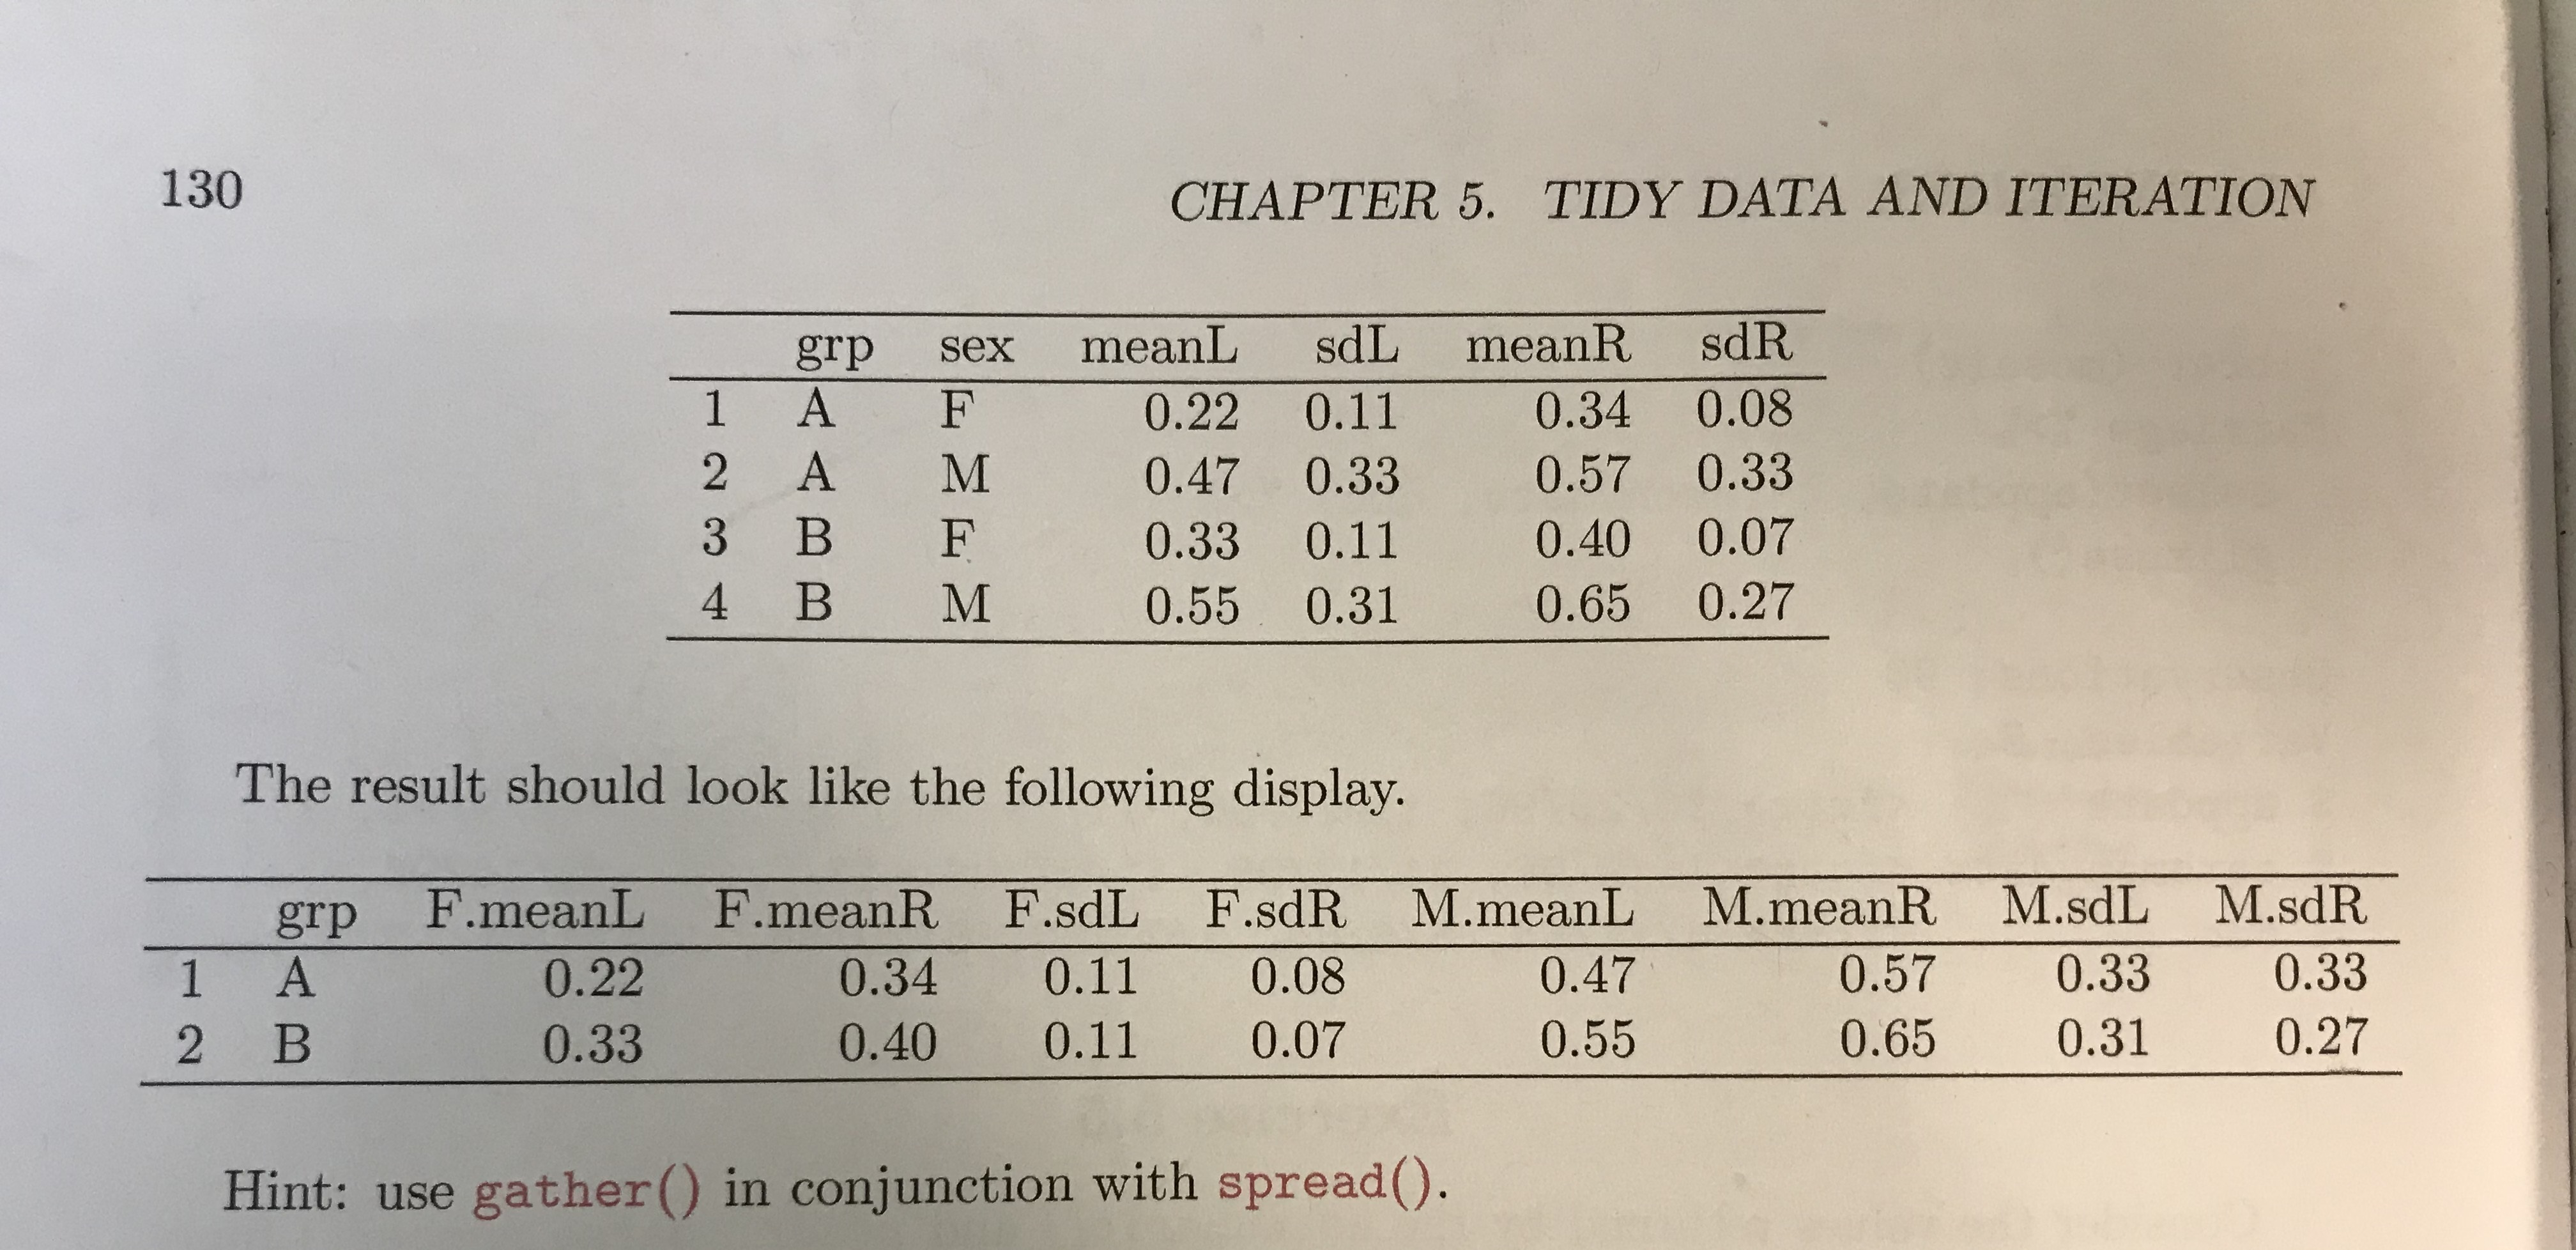
\includegraphics{images/mdsr_ex_5_7.jpg}

\begin{Shaded}
\begin{Highlighting}[]
\NormalTok{FakeDataLong }\OtherTok{\textless{}{-}} \FunctionTok{data.frame}\NormalTok{(}\AttributeTok{grp =} \FunctionTok{c}\NormalTok{(}\StringTok{"A"}\NormalTok{,}\StringTok{"A"}\NormalTok{,}\StringTok{"B"}\NormalTok{, }\StringTok{"B"}\NormalTok{)}
\NormalTok{                           , }\AttributeTok{sex =} \FunctionTok{c}\NormalTok{(}\StringTok{"F"}\NormalTok{, }\StringTok{"M"}\NormalTok{, }\StringTok{"F"}\NormalTok{, }\StringTok{"M"}\NormalTok{)}
\NormalTok{                           , }\AttributeTok{meanL =} \FunctionTok{c}\NormalTok{(}\FloatTok{0.22}\NormalTok{, }\FloatTok{0.47}\NormalTok{, }\FloatTok{0.33}\NormalTok{, }\FloatTok{0.55}\NormalTok{)}
\NormalTok{                           , }\AttributeTok{sdL =} \FunctionTok{c}\NormalTok{(}\FloatTok{0.11}\NormalTok{, }\FloatTok{0.33}\NormalTok{, }\FloatTok{0.11}\NormalTok{, }\FloatTok{0.31}\NormalTok{)}
\NormalTok{                           , }\AttributeTok{meanR =} \FunctionTok{c}\NormalTok{(}\FloatTok{0.34}\NormalTok{, }\FloatTok{0.57}\NormalTok{, }\FloatTok{0.40}\NormalTok{, }\FloatTok{0.65}\NormalTok{)}
\NormalTok{                           , }\AttributeTok{sdR =} \FunctionTok{c}\NormalTok{(}\FloatTok{0.08}\NormalTok{, }\FloatTok{0.33}\NormalTok{, }\FloatTok{0.07}\NormalTok{, }\FloatTok{0.27}\NormalTok{))}
\end{Highlighting}
\end{Shaded}

\begin{Shaded}
\begin{Highlighting}[]
\NormalTok{FakeDataLong1 }\OtherTok{\textless{}{-}}\NormalTok{ FakeDataLong }\SpecialCharTok{\%\textgreater{}\%}
\FunctionTok{gather}\NormalTok{(}\StringTok{"statistics"}\NormalTok{, }\StringTok{"value"}\NormalTok{, }\SpecialCharTok{{-}}\FunctionTok{c}\NormalTok{(}\StringTok{"grp"}\NormalTok{, }\StringTok{"sex"}\NormalTok{)) }\SpecialCharTok{\%\textgreater{}\%}
\FunctionTok{unite}\NormalTok{(sex.statistics, }\FunctionTok{c}\NormalTok{(}\StringTok{"sex"}\NormalTok{, }\StringTok{"statistics"}\NormalTok{), }\AttributeTok{sep =} \StringTok{"."}\NormalTok{) }\SpecialCharTok{\%\textgreater{}\%}
\FunctionTok{arrange}\NormalTok{(sex.statistics) }\SpecialCharTok{\%\textgreater{}\%}
\FunctionTok{spread}\NormalTok{(}\AttributeTok{key =} \StringTok{"sex.statistics"}\NormalTok{, }\AttributeTok{value =} \StringTok{"value"}\NormalTok{)}
\end{Highlighting}
\end{Shaded}

\newpage

\hypertarget{pug-brainstorming}{%
\section{PUG Brainstorming}\label{pug-brainstorming}}

What topics or questions are you interested in exploring related to your
PUG theme? Dream big here. Don't worry about whether there is data out
there that's available and accessible that you could use to address your
questions/topics. Just brainstorm some ideas that get you excited. Then,
email your PUG team with your ideas. Title the email ``PS2B
Brainstorming: PUG {[}\#{]} {[}Topic{]}'' and CC me
(\href{mailto:kcorreia@amherst.edu}{\nolinkurl{kcorreia@amherst.edu}})
on the email. If another PUG member already initiated the email, reply
all to their email.

If you don't remember your PUG \# and Topic, please see the file
``PUGs'' on the Moodle page under this week.

If you don't know your PUG members email address, go to the class's
Google group conversations (e.g., by clicking the link ``Link to Google
group conversations'' at the top of our Moodle course page). Then, on
the navigation panel (left hand side), select ``Members''.

\begin{quote}
ANSWER: Do not write anything here. Email your ideas to your PUG team
and me in a message titled ``PS2B Brainstorming: PUG {[}\#{]}
{[}Topic{]}''.
\end{quote}

\end{document}
